\documentclass[11pt]{article}
\usepackage[margin=1in]{geometry}
\usepackage{amsmath,amssymb,amsthm}
\usepackage{bm}
\usepackage{enumitem}
\usepackage[hidelinks]{hyperref}
\usepackage{booktabs}
\usepackage{graphicx}
\usepackage{caption}
\usepackage{subcaption}
\usepackage{xcolor}
\usepackage{longtable}
\usepackage{multirow}

\newtheorem{definition}{Definition}
\newtheorem{remark}{Remark}

% ==== convenience macros (shared with problem_formulation.tex) ====
\newcommand{\R}{\mathbb{R}}
\newcommand{\E}{\mathbb{E}}
\newcommand{\Fspace}{\mathcal{F}}
\newcommand{\gates}{\mathcal{G}}
\newcommand{\proto}{\Theta}
\newcommand{\evalop}{\mathcal{E}}
\newcommand{\zoo}{\Fspace_{\mathrm{zoo}}}
\newcommand{\combiner}{\mathcal{M}}
\newcommand{\main}{\textsc{main}}
\newcommand{\orig}{\textsc{original}}

\title{\vspace{-2.5em}\textbf{Mid-Research Report}\\[0.3em]
\large Does Outcome-Aware Evolution Learn?\\
A Controlled Comparison of a Learning-Aware Alpha Miner\\
Against Its Paper Baseline}
\date{\today}

\sloppy
\begin{document}
\maketitle
\vspace{-2em}

\section{Introduction}
\label{sec:intro}

This system uses a large language model to invent stock-picking formulas --- it
proposes a formula, tests it on historical market data, and repeats. The question is
whether the repetition helps. If each round's proposals are no better than the last,
the system is just a random generator with a language model attached, and the only
thing improving is the best of a growing pile of lucky guesses.

We compare two versions that differ in what happens \emph{after} a formula is tested.
The baseline (\orig{}, the original published method) proposes, tests, and keeps
everything. The treatment (\main{}) adds four things: a gate that only keeps a formula
if it improves the overall portfolio; a diagnosis step that works out \emph{why} a
formula failed and tells the generator; a mechanism to inject fresh ideas when
progress stalls; and a memory that carries failures across rounds. Both use the same
language model, the same market (China's CSI300), the same schedule, and ten ideas per
round.

Three differences between the two runs shape how the results must be read. Each was
measured, not assumed.

\begin{description}[leftmargin=0em,itemsep=0.25em,style=nextline]
\item[The same 150 formulas cost different effort (\S\ref{sub:budget}).]
  Both run the paper's ten ideas per round, but \orig{} turns each idea into three
  formulas --- as its published method specifies --- while \main{} turns each into one.
  Reaching 150 formulas therefore took \main{} 161 ideas and \orig{} only 60. A
  ``round'' means different things in each, so progress is measured per formula, and
  holding the formula count equal is generous to the baseline.
\item[The two runs were tuned on different eras (\S\ref{sec:learning}).]
  \main{}'s gate was calibrated on 2013--2015 and \orig{} on 2021, so a shared
  2022--2025 test sits seven years after one and one year after the other. This was an
  oversight in the setup, and it works against \main{}, whose formulas must survive six
  more years of drift.
\item[More formulas automatically score better (\S\ref{sub:count}).]
  The model that combines formulas into one signal improves simply from having more
  inputs, regardless of their quality. A 56-formula library and a 150-formula library
  therefore cannot be compared directly.
\end{description}

\noindent The report asks four questions: does the treatment build a better portfolio
(\S\ref{sec:results})? does it learn (\S\ref{sec:learning})? do its breeding operators
actually improve on what they breed from (\S\ref{sec:learning})? and does it deliver
the variety and trading capacity it was designed for
(\S\ref{sec:capacity}--\ref{sec:diversity})?

\paragraph{What we found.}
At equal formula count \main{}'s library builds a better portfolio than \orig{}'s, and
over 2017--2025 it leads on both backtests ($+35.5\%$ against $+20.9\%$ a year under
simple costs; $+9.6\%$ against $+3.1\%$ under realistic ones) with a higher prediction
score in all nine years and a smaller worst-case loss. It also has by far the best
trading capacity: run as a fund that starts at 100M and compounds, it beats the market
by $7.8\%$ a year where the baseline manages $2.4\%$, and it is the last library to
turn unprofitable as the fund grows.

Most directly, \main{} \emph{does} get better as it goes. Measured formula by formula
--- the one axis both systems share, since each mined exactly 150 --- the prediction
quality of what \main{} proposes rises by $0.0236$ Rank IC per hundred formulas,
against $+0.0038$ for the baseline: about six times faster. \main{} starts level with
\orig{} (Rank IC $0.031$ against $0.032$ over the first fifty) and finishes $53\%$
ahead ($0.055$ against $0.036$). Its breeding also beats the formulas it breeds from
$53$--$61\%$ of the time, where the baseline's does so \emph{less} often than chance.

The system's weak point is not the formulas. Over 2017--2025 they predict well and
consistently under a simple portfolio construction, yet the realistic-cost path turns
negative after 2020 --- and the two paths disagree on the \emph{prediction} score too,
which no cost model can explain. The component that combines many formulas into one
signal is where the value is lost, and that is what to fix next.

\section{Experimental Design}
\label{sec:design}

\subsection{The three libraries}

Both systems use the same language model, the same market, and the same schedule.
\orig{} keeps every formula it produces. \main{} keeps a formula only if it improves
the portfolio, so it ends up with two collections: everything it generated, and the
subset it chose to keep. Table~\ref{tab:libraries} names all three.

\begin{table}[h]
\centering\small
\begin{tabular}{llrl}
\toprule
Name & From & Count & What it is \\
\midrule
\main{}-full & \main{} & 150 & every formula \main{} generated \\
\main{}-kept & \main{} & 56  & the ones its quality gate kept --- what it would trade \\
\orig{}      & \orig{} & 150 & every formula \orig{} generated (it keeps all) \\
\bottomrule
\end{tabular}
\caption{The three collections of formulas compared throughout.
\textbf{Conclusion: the three isolate different questions} --- \orig{} against
\main{}-full tests the generators head to head at equal size, and \main{}-full against
\main{}-kept tests whether the quality gate earns its keep.}
\label{tab:libraries}
\end{table}

\noindent Three comparisons follow. \orig{} against \main{}-full asks whose
\emph{generator} is better (same count, neither filtered). \main{}-full against
\main{}-kept asks whether the \emph{gate} adds value. And \main{}-kept against
\orig{} asks how the portfolio \main{} would actually trade compares with the
baseline's whole pile.

\subsection{The same 150 formulas cost very different effort}
\label{sub:budget}

Both systems are set up identically and both generate ten ideas per round --- the
budget the published method specifies. The difference, quantified in
Table~\ref{tab:budget}, is what an idea produces: \orig{} turns each into three
formulas, \main{} into one.

This is deliberate on both sides. \orig{} is run \emph{exactly as its paper specifies},
three formulas per idea included, because the point of a baseline is to represent the
published method rather than a modernised version of it. \main{} spends the same budget
on one formula per idea, so that a failed idea is a failed \emph{idea} rather than one
of three variations that might succeed by chance. Neither is a defect in the setup; the
consequences below simply follow from it.

\begin{table}[h]
\centering\small
\begin{tabular}{lrr}
\toprule
& \main{} & \orig{} \\
\midrule
Ideas per round             & 10    & 10 \\
Formulas per idea           & 0.93  & 2.50 \\
Rounds to reach 150         & 18    & 6 \\
Distinct ideas explored     & \textbf{161} & \textbf{60} \\
Deepest breeding chain      & 5     & 5 \\
\bottomrule
\end{tabular}
\caption{Both systems run the paper's budget of ten ideas per round; they differ in how
many formulas an idea yields, with \orig{} following its published three-per-idea
specification. \textbf{Conclusion: reaching the same 150 formulas therefore cost
\main{} $2.7\times$ as many distinct ideas --- it spends its budget on new thinking
rather than on variations of the same thought.}}
\label{tab:budget}
\end{table}

\noindent Two consequences follow. A ``round'' is not a comparable unit (ten formulas
in \main{}, thirty in \orig{}), so progress is measured per formula and each system is
only ever compared with itself. And fixing the count at 150 is generous to \orig{},
which reaches it having committed to far fewer distinct ideas --- while the merging
model separately rewards simply having more formulas (\S\ref{sub:count}).

\subsection{Backtests and the no-leak window}
\label{sub:noleak}

Every library is tested twice, and both tests buy the same portfolio --- the 50
highest-scoring stocks each day, equally weighted --- so the only differences are how
the formulas are merged and how trading is charged.

\begin{enumerate}[leftmargin=1.6em,itemsep=0.15em]
  \item \textbf{The simple backtest} merges the formulas with a single model and
        charges a flat trading fee, regardless of how much money is being managed.
        This is the setup the original paper used.
  \item \textbf{The realistic backtest} merges them with a two-stage model and charges
        a fee that \emph{grows with position size}, reflecting the fact that large
        trades move prices against you. This is the one to believe for questions about
        real profitability.
\end{enumerate}

\begin{remark}[Neither system saw the test period]
Everything is scored on years that came after any data either system used to choose
its formulas. \orig{} selected on 2021 and earlier and in any case never filtered
anything; \main{}'s gate used data ending in 2015. Both backtests then train their own
merging model on earlier years before scoring the test period, so no result below is
contaminated by hindsight.
\end{remark}

\section{What the Numbers Mean}
\label{sec:metrics}

A \emph{formula} scores every stock each day; the \emph{portfolio} is built by buying
the 50 highest-scoring ones. Two questions matter: does the score predict what happens
next, and does trading on it make money after costs? Table~\ref{tab:metrics} defines
every measure used in this report, with the range it can take, what counts as good,
and what \main{} achieves.

\begin{table}[h]
\centering\footnotesize
\setlength{\tabcolsep}{3pt}
\renewcommand{\arraystretch}{1.12}
\begin{tabular}{@{}p{1.75cm}p{4.5cm}p{1.75cm}p{1.5cm}p{1.9cm}p{1.9cm}@{}}
\toprule
\textbf{Metric} & \textbf{What it means} & \textbf{Range} & \textbf{Good is} &
\textbf{\main{}} & \textbf{\orig{}} \\
\midrule
IC &
Do the stocks it ranks highest actually go up most? Measured within each day, so
market-wide moves cancel out. &
$-1$ to $1$; real $0.01$--$0.10$ &
$>0.03$ &
$\bm{0.118}$ & $0.105$ \\
Rank IC &
Same, using only the \emph{order} of scores. Since we buy the top 50, this is the
number that matters. &
$-1$ to $1$ &
$>0.03$ &
$\bm{0.114}$ & $0.101$ \\
Rank IC, one formula &
The same, for a single formula rather than the whole portfolio. &
$-1$ to $1$ &
$>0.02$ &
$\bm{0.046}$ & $0.034$ \\
Rank ICIR &
How \emph{consistent} the edge is day to day, rather than how big. &
usually $0$--$1$ &
$>0.3$; $>0.5$ strong &
$\bm{0.876}$ & $0.808$ \\
Annual return, simple &
Compound yearly rate after a flat trading fee. &
unbounded &
$>5\%$ excess &
$\bm{+35.5\%}$ & $+20.9\%$ \\
Annual return, realistic &
The same, once trading impact grows with size. &
unbounded &
$>5\%$ excess &
$\bm{+9.6\%}$ & $+3.1\%$ \\
Info.\ ratio &
Return per unit of risk. &
unbounded &
$>1$; $>2$ strong &
$\bm{4.00}$ & $2.51$ \\
Max drawdown &
Worst peak-to-trough loss along the way. &
$-100\%$ to $0$ &
better than $-20\%$ &
$\bm{-7.9\%}$ & $-10.6\%$ \\
Turnover &
Share of the portfolio traded daily --- the multiplier on every cost. &
$0$ to $1$ &
$<0.20$/day &
$0.106$ & $0.106$ \\
Cost &
Trading friction, in hundredths of a percent traded, at 100M. &
$\ge 0$ &
$<10$ &
$5.81$ & $\bm{5.49}$ \\
Capacity &
Excess return running a fund that starts at 100M and compounds. &
unbounded &
$>0$ &
$\bm{+7.84\%}$ & $+2.40\%$ \\
Effective rank &
How many genuinely \emph{different} ideas the library holds. 150 near-copies count as
far fewer. &
$1$ to $n$ &
$>20\%$ of $n$ &
$\bm{38}$ ($26\%$) & $36$ ($24\%$) \\
Redundancy &
Share of formula pairs too similar to each other. &
$0$ to $1$ &
low &
$\bm{4.4\%}$ & $5.1\%$ \\
Crash IC &
Does the edge survive the worst $20\%$ of market days? &
$-1$ to $1$ &
$\ge$ overall IC &
$0.054$ & $\bm{0.058}$ \\
Improvement &
Gain in formula quality per 100 formulas mined --- does it learn? &
unbounded &
$>0$ &
$\bm{+0.0236}$ & $+0.0038$ \\
\bottomrule
\end{tabular}
\caption{Every measure used in this report, and what each system achieves, over
2017--2025 for the full 150-formula libraries. Return, cost and capacity are from the
\textbf{realistic cost model} (trading impact grows with fund size), except the
``simple'' return row; prediction scores are unaffected by the cost model.
\textbf{Conclusion: \main{} is ahead on thirteen of fifteen measures} --- including
every measure of prediction, return, risk, capacity and learning rate. \orig{} leads
only on trading cost ($5.49$ against $5.81$ basis points) and on how well the edge
survives market crashes ($0.058$ against $0.054$); turnover ties. ``Good is'' are
conventional rules of thumb, not thresholds the system enforces.}
\label{tab:metrics}
\end{table}

\paragraph{Two ways of quoting a return.}
\emph{Excess} return subtracts the market, answering ``did the stock-picking add
anything?''. \emph{Net} return adds the market back, answering ``what did the money
actually earn?''. Every return table below shows the market's own return too, so
either can be read off. The two backtests measure the market slightly differently ---
the realistic-cost one corrects for dividends, the simple one does not --- so their
return columns are compared \emph{between libraries}, not against each other.

\section{Results}
\label{sec:results}
All numbers are computed on \textbf{2022-01-01 -- 2025-12-26}, out of sample for both
arms (\S\ref{sub:noleak}). Two independent backtests are reported because they
disagree, and the disagreement is informative.

\subsection{Per-year results}

Every library is scored by both backtests on 2022--2025, reported year by year:
Table~\ref{tab:bt2-2225} under simple costs, Table~\ref{tab:fc-2225} under realistic
ones.

\begin{table}[h]
\centering\small
\setlength{\tabcolsep}{5pt}
\begin{tabular}{llrrrrr}
\toprule
& & 2022 & 2023 & 2024 & 2025 & full \\
\midrule
\multirow{3}{*}{IC}
 & \main{}-kept (56)   & $0.0972$ & $0.0930$ & $0.0919$ & $0.0796$ & $0.0905$ \\
 & \main{}-full (150) & $\bm{0.1391}$ & $\bm{0.1337}$ & $\bm{0.1364}$ & $\bm{0.1116}$ & $\bm{0.1302}$ \\
 & \orig{} (150)      & $0.1060$ & $0.1247$ & $0.1195$ & $0.0902$ & $0.1101$ \\
\midrule
\multirow{3}{*}{Rank IC}
 & \main{}-kept   & $0.0938$ & $0.0921$ & $0.0917$ & $0.0756$ & $0.0883$ \\
 & \main{}-full  & $\bm{0.1364}$ & $\bm{0.1308}$ & $\bm{0.1339}$ & $\bm{0.1060}$ & $\bm{0.1268}$ \\
 & \orig{}       & $0.1024$ & $0.1227$ & $0.1157$ & $0.0856$ & $0.1066$ \\
\midrule
\multirow{3}{*}{Return}
 & \main{}-kept   & $34.81\%$ & $19.73\%$ & $13.84\%$ & $1.04\%$ & $16.76\%$ \\
 & \main{}-full  & $\bm{52.07\%}$ & $\bm{37.84\%}$ & $\bm{38.98\%}$ & $\bm{23.42\%}$ & $\bm{37.74\%}$ \\
 & \orig{}       & $29.24\%$ & $30.34\%$ & $33.41\%$ & $3.54\%$ & $23.55\%$ \\
\cmidrule(l){2-7}
 & \emph{CSI300 (price)} & $-21.7\%$ & $-11.4\%$ & $+14.7\%$ & $+17.7\%$ & $-1.4\%$ \\
 & \emph{CSI300 (total)} & $-20.4\%$ & $-10.1\%$ & $+16.5\%$ & $+19.1\%$ & $+0.9\%$ \\
\bottomrule
\end{tabular}
\caption{\textbf{Simple backtest} (flat trading fee), 2022--2025, at \textbf{100M CNY}
of capital. Returns are excess of the CSI300 price index, whose own return is shown
for reference. \textbf{Conclusion: \main{}-full leads \orig{} on every metric in every
year}, and both beat a market that fell over this period.}
\label{tab:bt2-2225}
\end{table}

\begin{table}[h]
\centering\small
\setlength{\tabcolsep}{5pt}
\begin{tabular}{llrrrrr}
\toprule
& & 2022 & 2023 & 2024 & 2025 & full \\
\midrule
\multirow{3}{*}{IC}
 & \main{}-kept (56)   & $0.0321$ & $0.0079$ & $0.0203$ & $0.0369$ & $0.0242$ \\
 & \main{}-full (147) & $\bm{0.0433}$ & $0.0151$ & $0.0294$ & $0.0394$ & $0.0318$ \\
 & \orig{} (149)      & $0.0347$ & $\bm{0.0276}$ & $\bm{0.0341}$ & $\bm{0.0408}$ & $\bm{0.0343}$ \\
\midrule
\multirow{3}{*}{Rank IC}
 & \main{}-kept   & $0.0433$ & $0.0194$ & $0.0306$ & $0.0569$ & $0.0375$ \\
 & \main{}-full  & $\bm{0.0598}$ & $0.0333$ & $0.0429$ & $\bm{0.0613}$ & $0.0493$ \\
 & \orig{}       & $0.0526$ & $\bm{0.0447}$ & $\bm{0.0481}$ & $0.0609$ & $\bm{0.0515}$ \\
\midrule
\multirow{4}{*}{Return}
 & \main{}-kept   & $-1.68\%$ & $-7.74\%$ & $-5.74\%$ & $-5.86\%$ & $-5.28\%$ \\
 & \main{}-full  & $\bm{+3.56\%}$ & $-2.83\%$ & $-3.60\%$ & $\bm{-6.38\%}$ & $\bm{-2.37\%}$ \\
 & \orig{}       & $-2.87\%$ & $\bm{-1.22\%}$ & $\bm{-0.75\%}$ & $-9.42\%$ & $-3.62\%$ \\
 & \emph{null model} & $-9.81\%$ & $-24.60\%$ & $-12.40\%$ & $-5.72\%$ & $-13.45\%$ \\
\cmidrule(l){2-7}
 & \emph{benchmark (EW, total)} & $-13.0\%$ & $-4.9\%$ & $+21.3\%$ & $+20.0\%$ & $+1.5\%$ \\
 & \emph{CSI300 (total)}        & $-20.4\%$ & $-10.1\%$ & $+16.5\%$ & $+19.1\%$ & $+0.9\%$ \\
\bottomrule
\end{tabular}
\caption{\textbf{Realistic-cost backtest} (trading impact grows with size),
2022--2025, at \textbf{100M CNY} of capital. Returns are excess of the benchmark
shown. The \emph{null model} is the identical machinery run with no mined formula in
it, so it isolates what the merging model and portfolio rule contribute on their own.
\textbf{Conclusion: nothing makes money on this window, but all three libraries beat
the null model by $8$--$11$ points --- the formulas carry genuine information, and the
machinery that trades them subtracts from it rather than supplying the edge.}}
\label{tab:fc-2225}
\end{table}

\noindent The two backtests disagree about which library is best, and the
disagreement is the point. Under simple costs \main{}-full leads in every year. Under
realistic costs \orig{} edges ahead on prediction in three of four years while
\main{}-full still leads on return --- \main{}'s formulas are cheaper to trade, so
they keep more of a smaller edge. Both agree that 2025 was the worst year for every
library, and that the 56-formula gated set scores below both 150-formula libraries,
for the reason \S\ref{sub:count} explains.

\paragraph{One correction was needed first.}
The realistic-cost setup measured the market using an index that \emph{excludes}
dividends, while the portfolio's own returns \emph{include} them --- which silently
credited the strategy with the market's dividend yield (about $4.25$ percentage points
a year) as if it were skill. Correcting it moved the gated set's return from $-2.4\%$
to $-5.3\%$ and the null model from $-11.0\%$ to $-13.5\%$. The prediction scores did
not move at all, since they compare stocks against each other on the same day and so
never see a market-wide effect.

\paragraph{What the null model is for.}
The \emph{null model} row runs the identical machinery --- the same merging model, the
same top-50 portfolio, the same cost charges --- on the base price and volume data
alone, with \emph{no mined formula in it}. It exists to answer an obvious objection:
if the whole pipeline made money, how would we know the edge came from the discovered
formulas rather than from the machinery that trades them? The null model measures
exactly that machinery on its own. It returns $-13.45\%$ a year, so the machinery by
itself destroys value; anything above that line is attributable to the formulas.

\paragraph{The headline.}
No library makes money on 2022--2025. All three still beat the null model by $8$--$11$
percentage points, so the formulas do carry real information --- the machinery is not
the source of the edge, and in fact subtracts from it. Over 2017--2025
(\S\ref{sub:long}) the same libraries are profitable for four consecutive years, so
this negative result belongs to the recent period rather than to the method.

\subsection{The long window: 2017--2025}
\label{sub:long}

The 2022--2025 window is short. Both backtests were re-run over 2017--2025
(Table~\ref{tab:long}), with the merging model fitted on 2005--2012 and checked on
2013--2015. This window overlaps \orig{}'s own 2021 test year, so it favours the
baseline rather than \main{}.

\begin{table}[h]
\centering\small
\setlength{\tabcolsep}{3.5pt}
\begin{tabular}{lrrrrrrrrrr}
\toprule
& 2017 & 2018 & 2019 & 2020 & 2021 & 2022 & 2023 & 2024 & 2025 & full \\
\midrule
\multicolumn{11}{l}{\emph{Simple backtest --- annual return}} \\
\main{}-full & $\bm{40.8}$ & $\bm{60.8}$ & $\bm{18.9}$ & $\bm{29.4}$ & $\bm{48.5}$ & $\bm{54.2}$ & $\bm{30.4}$ & $28.6$ & $\bm{14.7}$ & $\bm{35.5}$ \\
\orig{}      & $3.8$ & $29.9$ & $8.2$ & $21.1$ & $33.7$ & $33.7$ & $26.2$ & $\bm{32.0}$ & $5.4$ & $20.9$ \\
\main{}-kept  & $8.4$ & $37.2$ & $5.8$ & $13.3$ & $29.8$ & $30.4$ & $20.3$ & $12.9$ & $10.1$ & $18.2$ \\
\midrule
\multicolumn{11}{l}{\emph{Simple backtest --- prediction (Rank IC)}} \\
\main{}-full & $\bm{.130}$ & $\bm{.126}$ & $\bm{.102}$ & $\bm{.112}$ & $\bm{.099}$ & $\bm{.125}$ & $\bm{.114}$ & $\bm{.123}$ & $\bm{.091}$ & $\bm{.114}$ \\
\orig{}      & $.108$ & $.109$ & $.092$ & $.096$ & $.093$ & $.103$ & $.111$ & $.110$ & $.084$ & $.101$ \\
\main{}-kept  & $.093$ & $.099$ & $.077$ & $.076$ & $.074$ & $.089$ & $.071$ & $.078$ & $.071$ & $.081$ \\
\midrule
\multicolumn{11}{l}{\emph{Realistic backtest --- annual return}} \\
\main{}-full & $\bm{52.8}$ & $\bm{41.0}$ & $\bm{19.8}$ & $17.8$ & $-5.9$ & $\bm{-2.0}$ & $-5.3$ & $-8.1$ & $-7.0$ & $\bm{9.6}$ \\
\orig{}      & $20.4$ & $18.7$ & $5.1$ & $\bm{18.4}$ & $\bm{-2.5}$ & $-7.9$ & $\bm{-3.7}$ & $\bm{-5.4}$ & $-9.7$ & $3.1$ \\
\main{}-kept  & $31.8$ & $35.5$ & $7.1$ & $8.9$ & $-5.0$ & $-8.2$ & $-10.1$ & $-10.2$ & $\bm{-6.4}$ & $3.6$ \\
\emph{null}  & $-4.9$ & $-12.2$ & $5.7$ & $-4.8$ & $-7.6$ & $-14.4$ & $-26.5$ & $-16.5$ & $-4.7$ & $-10.0$ \\
\midrule
\multicolumn{11}{l}{\emph{Realistic backtest --- prediction (Rank IC)}} \\
\main{}-full & $\bm{.155}$ & $\bm{.156}$ & $\bm{.132}$ & $\bm{.131}$ & $\bm{.055}$ & $\bm{.060}$ & $.033$ & $.043$ & $\bm{.061}$ & --- \\
\orig{}      & $.123$ & $.126$ & $.107$ & $.110$ & $.054$ & $.053$ & $\bm{.045}$ & $\bm{.048}$ & $.060$ & --- \\
\main{}-kept  & $.127$ & $.127$ & $.109$ & $.099$ & $.047$ & $.043$ & $.019$ & $.031$ & $.056$ & --- \\
\midrule
\multicolumn{11}{l}{\emph{Benchmarks}} \\
\emph{bench (EW, total)} & $8.0$ & $-26.6$ & $35.8$ & $27.3$ & $7.5$ & $-13.0$ & $-4.9$ & $21.3$ & $20.0$ & $6.6$ \\
\emph{CSI300 (total)}    & $24.1$ & $-23.8$ & $38.6$ & $29.8$ & $-3.7$ & $-20.4$ & $-10.1$ & $16.5$ & $19.1$ & $5.6$ \\
\bottomrule
\end{tabular}
\caption{Both backtests, 2017--2025, at \textbf{100M CNY} of capital. Returns are
compound annual growth rates in \%, so the ``full'' column is the rate that, compounded
over the nine years, reproduces the actual result. The simple backtest does not correct
for dividends, so its return rows compare between libraries rather than against the
realistic ones. \textbf{Conclusion: \main{}-full leads on both backtests and predicts
better in all nine years; but the two disagree sharply after 2020 --- profitable
throughout under simple costs, negative from 2021 under realistic ones --- and they
disagree on prediction too, which points at the merging model rather than the
formulas.}}
\label{tab:long}
\end{table}

\paragraph{The two backtests disagree, and that locates the problem.}
Under simple costs \main{}-full makes money in all nine years and predicts better than
\orig{} in every one. Under realistic costs the same library is profitable only
through 2020 and loses money from 2021.

Costs cannot explain a gap that large, because the two also disagree on the
\emph{prediction} score --- and prediction has no cost model in it at all. On
identical formulas over identical days, the simple path measures $0.09$--$0.13$ after
2020 while the realistic path drops to $0.03$--$0.06$. Nor is it how the portfolio is
built: both buy the top 50 stocks, equally weighted, with no position limits. The one
thing that differs is the \emph{combiner} --- the model that merges many formulas into
a single score. Since prediction is measured on the combiner's output, that is what
the gap points to.

This is not evidence that the strategy is profitable; the realistic path is the one to
believe, and it says otherwise after 2020. It is evidence that the problem is not the
formulas: they predict well and steadily across the whole period when merged by the
simpler model. The combiner is what to fix before judging the formulas' economic
worth.

\subsection{The count confound, and what it hides}
\label{sub:count}

Taken at face value, Table~\ref{tab:fc-2225} says \orig{} predicts best (Rank IC
$0.052$) ahead of \main{}-full (Rank IC $0.049$), with the 56-formula kept set last
(Rank IC $0.038$) --- so being selective looks like a mistake. That comparison is
invalid. The combiner gets one input per formula and improves simply from having more
inputs, whether or not the extra ones are any good. Scoring random subsets of a
\emph{single} library makes this obvious (Table~\ref{tab:count-curve}):

\begin{table}[h]
\centering\small
\setlength{\tabcolsep}{4pt}
\begin{tabular}{lrrrrrrr}
\toprule
$n$ & 10 & 20 & 40 & 56 & 80 & 120 & full \\
\midrule
\textsc{main-full} Rank IC & $0.0232$ & $0.0344$ & $0.0388$ & $0.0452$ & $0.0478$ & $0.0483$ & $0.0493$ \\
\textsc{original} Rank IC & $0.0288$ & $0.0384$ & $0.0391$ & $0.0441$ & $0.0505$ & $0.0501$ & $0.0515$ \\
\bottomrule
\end{tabular}
\caption{Prediction quality against the number of formulas fed to the merging model,
within a single library (2022--2025, 100M CNY, realistic cost model).
\textbf{Conclusion: prediction rises with count alone, so libraries of different sizes
cannot be compared directly --- any comparison that does not hold the count fixed
penalises the more selective system.}}
\label{tab:count-curve}
\end{table}

\noindent Holding the count fixed at 56 --- the size of \main{}'s kept set --- and
drawing five random 56-formula subsets of each 150-formula library gives the
like-for-like comparison in Table~\ref{tab:count-matched}:

\begin{table}[h]
\centering\small
\begin{tabular}{lrr}
\toprule
Arm at $n=56$ & Rank IC & Return \\
\midrule
\main{} gated zoo (the actual book)   & $0.0375$          & $\bm{-5.28\%}$ \\
\orig{} subsets (mean $\pm$ sd)       & $\bm{0.0395 \pm 0.0011}$ & $-7.43\%$ \\
\main{}-full subsets (mean $\pm$ sd)  & $0.0462 \pm 0.0021$ & $-4.80\%$ \\
\bottomrule
\end{tabular}
\caption{Like-for-like comparison at 56 formulas each (2022--2025, 100M CNY, realistic
cost model), using five random draws from the two 150-formula libraries.
\textbf{Conclusion: at equal size \main{}'s generator wins clearly ($+0.007$ prediction,
$+2.6$ points of return, no overlap across draws); its quality gate beats the baseline
on return but roughly ties a random draw from \main{}'s own library.}}
\label{tab:count-matched}
\end{table}

\noindent Two things follow. First, on the \emph{generator} question --- comparing the
two unfiltered libraries at equal size --- \main{} wins on both measures: prediction
(Rank IC $0.046$ against $0.040$) and annual return ($-4.80\%$ against $-7.43\%$, a
$2.6$-point lead), with no overlap across the five draws. \orig{}'s apparent lead at
full size was purely the count effect.

Second, on the \emph{gate} question, the right comparison is against what the gate is
for. It selects formulas that improve the portfolio's \emph{return}, not formulas that
predict best in isolation. Against the baseline at the same size it does exactly that:
it gives up $0.002$ of prediction (Rank IC $0.038$ against $0.040$) and gains $2.2$
points of annual return ($-5.28\%$ against $-7.43\%$). Judged on the quantity it
optimises, the gate works.

Its limitation is narrower than that trade suggests. Against a random 56 drawn from
\main{}'s \emph{own} library the gate is roughly a wash --- slightly behind on both
prediction (Rank IC $0.038$ against $0.046$) and return ($-5.28\%$ against $-4.80\%$).
So the gate adds real value over the baseline's formulas, but it does not yet beat
simply taking a random handful of \main{}'s own. Given that its selections were made
under a merging model whose prediction quality collapses after 2020
(\S\ref{sub:long}), that is what one would expect: the gate is choosing well against a
scoring function that is itself degraded. Fixing the merging model is the prerequisite
for testing the gate properly.

One measure does favour \orig{}: judged one formula at a time rather than as a
portfolio, its formulas are stronger (average Rank IC of $0.013$ against $0.011$).
That is the same trade seen from the other side ---
\main{}'s formulas combine better, \orig{}'s stand alone better.


\section{Does the System Learn?}
\label{sec:learning}

\subsection{Definition, and how it is measured fairly}

A generator cannot produce a strictly better formula every time; demanding that sets a
bar no search meets. The definition, fixed before measurement:

\begin{definition}[Learning]
\label{def:learning}
A system learns from its mistakes and successes if, as the search progresses,
\textbf{(L1)} it does not get worse --- the quality of what it proposes is flat or
rising; \textbf{(L2)} the set it keeps improves; and \textbf{(L3)} the best result so
far keeps rising.
\end{definition}

\noindent Two choices make the comparison fair, both following from the fact that
\orig{} is run exactly as its paper specifies (\S\ref{sub:budget}) rather than being
adjusted to match \main{}.

\textbf{Progress is measured per formula, not per round.} Because the published method
yields three formulas per idea and \main{} yields one, a round is ten formulas in
\main{} and thirty in \orig{} --- so anything ``per round'' would compare different
quantities. Both libraries contain exactly 150 formulas mined in order, which is a
common axis.

\textbf{Each system is scored on the metric it recorded itself}, in its own library
file, on its own evaluation window. Absolute levels are therefore never compared across
systems --- only the \emph{slope} of each system against itself, which is precisely the
question ``does it get better as it goes?''. Both libraries record prediction quality
(Rank IC) per formula, so that is the shared measure.

\subsection{Do the formulas get better?}

\begin{table}[h]
\centering\small
\begin{tabular}{llrrr}
\toprule
System & Measure & Change per 100 formulas & First third $\to$ last third & $p$ \\
\midrule
\main{} & Rank IC & $\bm{+0.0236}$ & $0.0311 \to \bm{0.0545}$ ($+75\%$) & $<0.001$ \\
\main{} & IC      & $+0.0126$ & $0.0080 \to 0.0209$ ($+161\%$) & $<0.001$ \\
\orig{} & Rank IC & $+0.0038$ & $0.0324 \to 0.0357$ ($+10\%$) & $<0.001$ \\
\orig{} & IC      & $+0.0030$ & $0.0144 \to 0.0165$ ($+15\%$) & $<0.001$ \\
\midrule
\main{} & Rank IC of the kept set & $+0.0617$ & $0.0314 \to 0.0545$ & $<0.001$ \\
\bottomrule
\end{tabular}
\caption{Improvement in formula quality across the 150 formulas each system mined, each
scored on its own recorded numbers so only slopes are compared, never levels. Every
trend survives a permutation test against shuffled ordering.
\textbf{Conclusion: both systems learn, but \main{} learns roughly six times faster
($+0.0236$ against $+0.0038$ per hundred formulas), and the formulas it keeps improve
faster still.}}
\label{tab:perfactor}
\end{table}

\noindent Table~\ref{tab:perfactor} is the central evidence that the system learns.
\main{} begins level with the baseline --- its first fifty formulas average a Rank IC
of $0.031$ against \orig{}'s $0.032$ --- and ends $53\%$ ahead ($0.055$ against
$0.036$). The rank correlation between formula number and quality is $+0.83$ for
\main{} against $+0.44$ for \orig{}, so the improvement is steady rather than driven by
a few late outliers. Figure~\ref{fig:learning} plots it.

\begin{figure}[h]
\centering
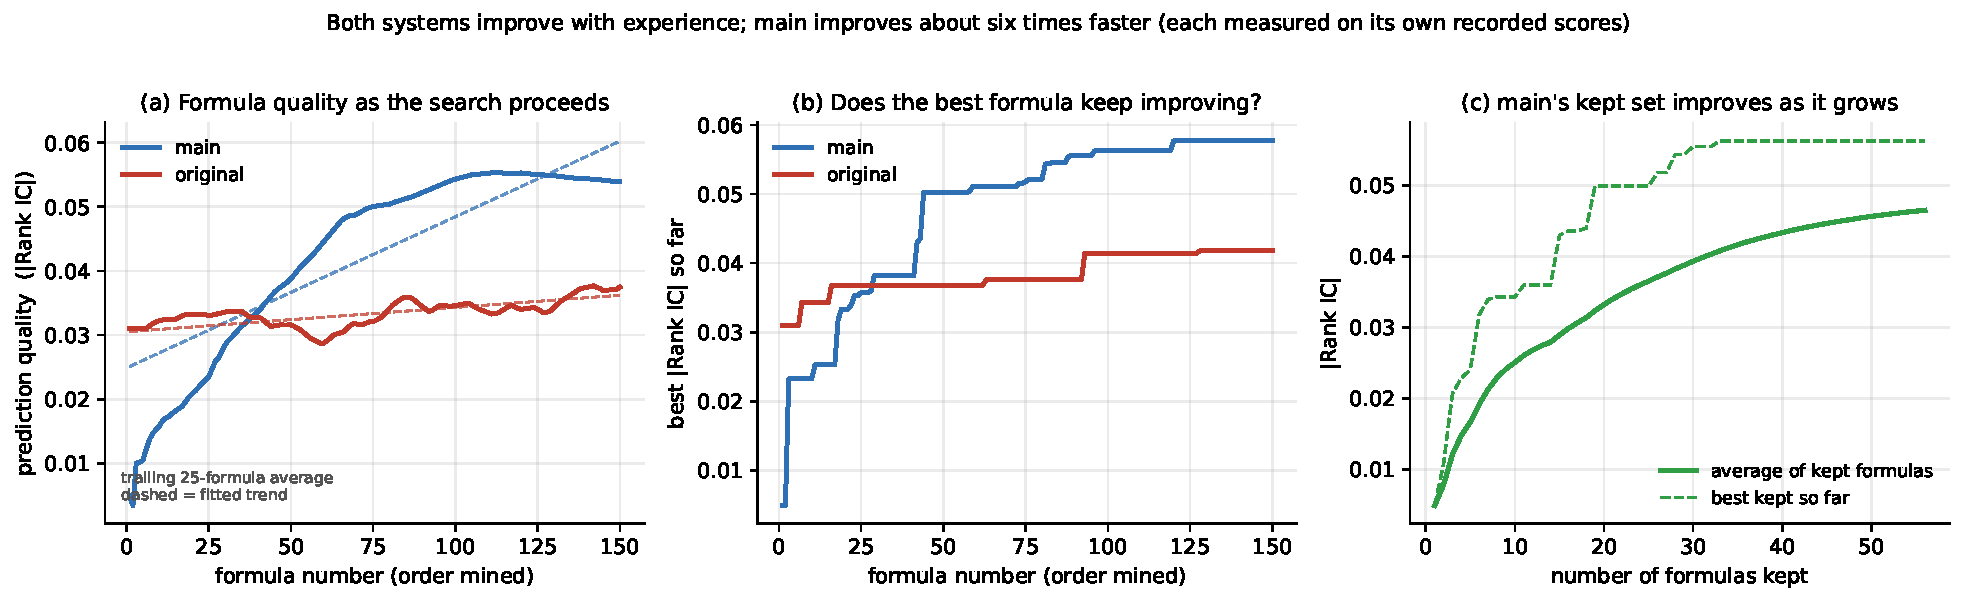
\includegraphics[width=\textwidth]{figures/fig_learning.pdf}
\caption{Left: formula quality against the order formulas were mined (trailing
25-formula average, dashed lines the fitted trends). Middle: the best formula found so
far. Right: \main{}'s kept set as it grows.}
\label{fig:learning}
\end{figure}

\noindent Two caveats. \main{}'s size-neutralised prediction score --- which strips out
any part of the edge explained by simply favouring small stocks --- rises more modestly
and is not statistically distinguishable from flat ($+0.0028$ per 100 formulas,
$p=0.31$), though its first-to-last-third comparison is positive ($0.0201 \to 0.0248$,
$p=0.041$). And formula quality here is each system's own recorded score, so the two
columns answer ``did this system improve?'' and not ``whose formulas are better?'' ---
that question is answered at equal count in \S\ref{sub:count}.

\subsection{Lineage: do the operators improve on their parents?}

New formulas are bred from old ones, so we can ask directly whether a child beats its
parent. Both systems record this fully (\main{} 161 formulas with 155 parent links,
\orig{} 60 with 37). A ``mutation'' has one parent, so beating it is a coin flip at
$50\%$; a ``crossover'' has two, so beating \emph{both} is about $33\%$ by chance.
Parents are already the stronger formulas in both systems, which makes the true bar
lower still.

\begin{table}[h]
\centering\small
\begin{tabular}{llrrrr}
\toprule
Operator & Metric & \main{} & \orig{} & chance & $n$ (\main{}/\orig{}) \\
\midrule
mutation  & Rank IC   & $\bm{61.3\%}$\,$(p{=}0.049)$ & $27.6\%$ & $50\%$ & 62 / 29 \\
mutation  & Rank ICIR & $56.5\%$ & $27.6\%$ & $50\%$ & 62 / 29 \\
mutation  & IC        & $50.0\%$ & $31.0\%$ & $50\%$ & 62 / 29 \\
\midrule
crossover & IC        & $\bm{58.1\%}$ & $21.1\%$ & $33\%$ & 43 / 19 \\
crossover & Rank IC   & $\bm{55.8\%}$ & $26.3\%$ & $33\%$ & 43 / 19 \\
crossover & ICIR      & $\bm{55.8\%}$ & $21.1\%$ & $33\%$ & 43 / 19 \\
\bottomrule
\end{tabular}
\caption{How often a newly bred formula beats the one(s) it was bred from, on each
system's own recorded prediction scores. \textbf{Conclusion: \main{}'s breeding
consistently beats chance ($53$--$61\%$ against bars of $33$--$50\%$), while \orig{}'s
falls \emph{below} it ($21$--$28\%$) --- its breeding usually destroys value.}}
\label{tab:lineage}
\end{table}

\noindent Table~\ref{tab:lineage} is the sharpest contrast in the report. Measured on
prediction quality (Rank IC), \main{}'s mutation produces a better formula than its
single parent $61.3\%$ of the time against a $50\%$ coin-flip bar, and its crossover
beats \emph{both} parents $53.5$--$58.1\%$ of the time against a $33\%$ bar --- roughly
$1.7\times$ chance. \orig{}'s mutation manages $27.6\%$ on the same measure, so its
bred formulas are usually \emph{worse} than what they came from. That is what breeding
without reading the results looks like.

\subsection{Verdict on the three tests}

\begin{table}[h]
\centering\small
\begin{tabular}{lll}
\toprule
& \main{} & \orig{} \\
\midrule
(L1) does not get worse & \textbf{PASS} --- rises, $p{<}0.001$ & \textbf{PASS} --- rises, $p{<}0.001$ \\
(L2) the kept set improves & \textbf{PASS} --- $+0.062$ per 100 kept & \textbf{N/A} --- keeps everything \\
(L3) the best keeps rising & \textbf{PASS} --- $0.023 \to 0.058$ & \textbf{PARTIAL} --- $0.031 \to 0.042$ \\
\midrule
Rate of improvement & $\bm{+0.0236}$ per 100 & $+0.0038$ per 100 \\
\bottomrule
\end{tabular}
\caption{The three learning tests, measured per formula on each system's own recorded
prediction quality (Rank IC). \textbf{Conclusion: \main{} passes all three; \orig{}
passes the first, partially passes the third, and cannot be scored on the second
because it keeps every formula it produces.}}
\label{tab:learning-verdict}
\end{table}

\noindent Table~\ref{tab:learning-verdict} scores all three. Both systems pass the
first --- neither degrades. The difference is rate: \main{} improves about six times
faster, and only \main{} has a kept set whose quality can improve, because \orig{}
keeps everything it produces.

Beyond prediction quality, \main{} records fourteen further measures the baseline
never computes, and twelve improve significantly as the gate keeps formulas: its own
portfolio-contribution score ($U$) from $0.55$ to $0.62$, the statistical strength of
new additions ($t$-statistic) from $3.9$ to $6.3$, and the stability score from $0.50$
to $0.98$. Every best-so-far record rises, and all of this happens while the bar for
statistical significance is \emph{tightening}, because testing more ideas demands
stronger evidence. All 29 replacements beat the formula they displaced on that same
$t$-statistic, and no formula was ever kept whose real behaviour contradicted the
economic story it claimed. Two measures worsen: formulas grow more similar to one
another (the highest correlation against an existing formula rises from $0.00$ to
$0.68$) and decay faster --- the price of buying variety.

\section{Trading Capacity}
\label{sec:capacity}

Market impact is the only cost term that scales with position size, so this applies to
the full-cost path alone (Backtest~v2 charges a flat fee, which is size-independent).
Participation is the traded weight divided by the stock's average daily volume as a
weight, so raising capital raises impact quadratically. Each library was re-priced at
100M, 500M and 1B CNY on both windows.

\paragraph{Are profits reinvested? Yes --- and it costs the strategy.}
The portfolio is always fully invested: each day every holding grows or shrinks with
its own gain or loss, and the positions are rescaled to add up to the whole fund, so
profits change \emph{what} is held. That means a fund that makes money gets bigger, and
a bigger fund pays more to trade, because its orders are larger relative to daily
volume.

A run labelled ``100M'' could be charged two ways: as a fund permanently held at 100M,
or as a fund that \emph{starts} at 100M and compounds. Table~\ref{tab:capacity} reports
both. In the compounding version the fund's value is carried forward day by day at its
own realised return, and each day's trading is charged against that running value ---
so growth raises the cost, which slows further growth.

\begin{table}[h]
\centering\small
\setlength{\tabcolsep}{3.5pt}
\begin{tabular}{lrrrrrrrrr}
\toprule
& \multicolumn{3}{c}{100M CNY} & \multicolumn{3}{c}{500M CNY} & \multicolumn{3}{c}{1B CNY} \\
\cmidrule(lr){2-4}\cmidrule(lr){5-7}\cmidrule(lr){8-10}
& held & compnd. & grew & held & compnd. & grew & held & compnd. & grew \\
\midrule
\multicolumn{10}{l}{\emph{2017--2025, excess return (\%\,a year)}} \\
\main{}-full & $+10.18$ & $\bm{+7.84}$ & $3.6\times$ & $+5.57$ & $\bm{+2.16}$ & $2.2\times$ & $+2.25$ & $\bm{-1.20}$ & $1.6\times$ \\
\main{}-kept & $+4.14$ & $+2.76$ & $2.3\times$ & $-0.30$ & $-2.10$ & $1.5\times$ & $-3.51$ & $-5.03$ & $1.1\times$ \\
\orig{}      & $+3.60$ & $+2.40$ & $2.3\times$ & $-1.10$ & $-2.47$ & $1.5\times$ & $-4.48$ & $-5.41$ & $1.1\times$ \\
\midrule
\multicolumn{10}{l}{\emph{2017--2025, net return (\%\,a year)}} \\
\main{}-full & $+17.18$ & $\bm{+14.69}$ & & $+12.29$ & $\bm{+8.65}$ & & $+8.75$ & $\bm{+5.09}$ & \\
\main{}-kept & $+10.71$ & $+9.24$ & & $+5.99$ & $+4.08$ & & $+2.58$ & $+0.96$ & \\
\orig{}      & $+10.14$ & $+8.87$ & & $+5.15$ & $+3.69$ & & $+1.56$ & $+0.56$ & \\
\midrule
\multicolumn{10}{l}{\emph{Trading cost (basis points), compounding}} \\
\main{}-full & $4.93$ & $5.81$ & & $6.68$ & $8.04$ & & $8.00$ & $9.41$ & \\
\bottomrule
\end{tabular}
\caption{Annual return at three fund sizes, realistic-cost backtest, 2017--2025.
``held'' charges trading as though the fund never changes size; ``compnd.'' lets the
fund grow at its own return and charges each day against its actual size; ``grew'' is
how many times over the fund multiplied. \emph{Excess} return subtracts the market
(which returned $6.60\%$ a year); \emph{net} is the return on the money itself.
\textbf{Conclusion: \main{}-full has much the best capacity at every size, but letting
the fund compound costs $1$--$3.5$ points a year and moves its practical ceiling from
beyond 1B to between 500M and 1B.}}
\label{tab:capacity}
\end{table}

\noindent Compounding costs $1$--$3.5$ percentage points a year, and it costs the most
where the fund grows the most: \main{}-full multiplies $3.6\times$ at 100M and gives up
$2.3$ points, and $3.4$ points at 500M and 1B. The effect is self-limiting --- a fund
that grows pays more, which slows its growth --- which is why the multiple falls from
$3.6\times$ at 100M to $1.6\times$ at 1B.

One headline changes. Under the fixed-size convention \main{}-full still beat the
market at 1B ($+2.25\%$); once the fund is allowed to compound, it does not
($-1.20\%$). Its practical ceiling is therefore somewhere between 500M and 1B rather
than beyond 1B. The ordering between systems is unchanged at every size, and every
library remains positive on a \emph{net} basis at every size --- \main{}-full earns
$+5.09\%$ a year even at 1B --- because the market itself returned $6.60\%$ over this
period.

\paragraph{Reading the curve.}
\main{}-full has the best capacity at every size, and by a wide margin: on the
compounding basis it beats \orig{} by $5.4$ percentage points of excess return at
100M, $4.6$ at 500M and $4.2$ at 1B. Its formulas are therefore cheaper to trade as
well as more predictive. Every library loses ground as size rises --- roughly $8$
points of excess return between 100M and 1B, with trading cost climbing from about
$4.9$ to $9.4$ basis points while the amount traded stays the same. The practical
ceiling sits near 100M for \orig{} and \main{}-kept, which turn negative by 500M, and
between 500M and 1B for \main{}-full.

\paragraph{On the shorter 2022--2025 window, nothing works at any size.}
There, excess returns run from $-2.4\%$ to $-11.5\%$ depending on library and size, and
the market itself returned almost nothing --- the equal-weight benchmark gained
$1.49\%$ a year and CSI300 $0.95\%$ (or $-1.36\%$ ignoring dividends), after falling
$20.4\%$ in 2022 and $10.1\%$ in 2023. With no market gain to lift the portfolio, the
net figures stay negative too.

\section{Diversity and Regime Behaviour}
\label{sec:diversity}

\main{}'s quality gate was built to buy \emph{variety} --- it rejects a formula that
closely resembles one already kept, or that adds no genuinely new information --- and
its feedback reports separately how each formula behaves when markets crash and when
they rally. Both are testable design claims, and Table~\ref{tab:diversity} tests them.
Similarity is judged with the gate's own threshold and its own correlation measure, so
both libraries face the identical bar the gate applied.

\begin{table}[h]
\centering\small
\begin{tabular}{lrrr}
\toprule
& \main{}-kept (56) & \main{}-full (147) & \orig{} (149) \\
\midrule
\multicolumn{4}{l}{\emph{Diversity / redundancy}} \\
Mean pairwise $|\rho|$        & $0.375$ & $0.215$ & $\bm{0.190}$ \\
Share of pairs $\ge \rho_{\text{bar}}$ & $15.5\%$ & $\bm{4.4\%}$ & $5.1\%$ \\
Effective rank                & $12.6$ & $\bm{38.1}$ & $36.0$ \\
Rank density (per factor)     & $22\%$ & $\bm{26\%}$ & $24\%$ \\
Distinct operators used       & $25$ & $\bm{28}$ & $25$ \\
Effective operators (evenness)& $16.4$ & $\bm{18.3}$ & $13.6$ \\
\midrule
\multicolumn{4}{l}{\emph{Regime behaviour}} \\
Mean $|$IC$|$, crash days     & $0.0484$ & $0.0540$ & $\bm{0.0576}$ \\
Mean $|$IC$|$, rally days     & $\bm{0.0460}$ & $0.0451$ & $0.0430$ \\
Crash-to-overall ratio        & $\bm{5.52}$ & $4.35$ & $4.43$ \\
Share whose edge survives a crash & $89\%$ & $88\%$ & $\bm{90\%}$ \\
\bottomrule
\end{tabular}
\caption{Variety and behaviour in bad markets (2022--2025, 100M CNY of capital,
realistic cost model). Similarity is judged with the same threshold the quality gate
itself uses. ``Crash'' and ``rally'' days are the worst and best $20\%$ of days for the
market as a whole. \textbf{Conclusion: the variety claim holds --- \main{} carries more
independent ideas and spreads them more evenly across building blocks --- but the
crash-robustness claim does not: \orig{} is marginally better on both crash measures.}}
\label{tab:diversity}
\end{table}

\paragraph{Diversity: the design claim holds, modestly.}
At equal size \main{}-full carries more independent directions than \orig{}
(effective rank $38.1$ against $36.0$, $26\%$ against $24\%$ of its factor count) and
fewer redundant pairs above the gate's threshold ($4.4\%$ against $5.1\%$). The
clearest margin is in \emph{operator evenness}: both libraries touch a similar number
of operator families, but \main{}'s usage is spread far more evenly ($18.3$ effective
operators against $13.6$), meaning \orig{} leans much harder on a few favourites.
That is what a search penalised for redundancy and rewarded for breadth should look
like. The margins are real but not large, and \main{} does not lead on mean pairwise
correlation.

The gated zoo is the interesting case: with only 56 factors it is markedly
\emph{more} internally correlated ($0.375$ mean, $15.5\%$ of pairs above threshold)
and carries an effective rank of $12.6$. Selecting for marginal contribution does not
produce a mutually orthogonal set --- it produces a set whose members each added
something \emph{at the moment they were admitted}, against a book that was smaller
then. This is the same breadth--purity cost visible in $\rho_{\max}$ rising from
$0.00$ to $0.68$ over the run (\S\ref{sec:learning}).

\paragraph{Regime robustness: not demonstrated.}
Every library shows a much stronger edge on crash days than on average --- crash
$|$IC$|$ is four to five times the all-day figure, and roughly nine in ten factors
retain their edge when markets fall. But \main{} does not lead: \orig{}'s crash
$|$IC$|$ is slightly higher ($0.0576$ against $0.0540$) and marginally more of its
factors survive a crash ($90\%$ against $88\%$). Reporting crash and rally IC to the
generator has not yet produced a measurably more crash-robust library. The
instrumentation exists; the search has not exploited it.

\section{Mechanisms}
\label{sec:mechanisms}

Both systems breed new formulas the same way: a first round proposes fresh ideas, then
rounds alternate between \emph{mutation} (tweak one formula) and \emph{crossover}
(combine two). The names match; what happens inside them does not.
Table~\ref{tab:mechanisms} summarises the differences described below.

\subsection{Which formulas get bred}

\paragraph{Choosing what to mutate.}
\orig{} takes every formula from the previous round, sorts them by an arbitrary index
number, and mutates all of them in that order. No measure of how well a formula
performed enters the choice.

\main{} sorts each formula by \emph{what its test result said}. A formula that failed
in a way the system can pin down is sent for repair --- breed a child that fixes that
specific defect. One that failed for no identifiable reason, or whose obvious repair
has already been tried, is abandoned in favour of a fresh start. A formula that
succeeded is used as breeding stock, and a share of the winners also get pushed
further in the same direction. Repairing failures takes priority over pushing winners.

\paragraph{Choosing crossover pairs.}
\orig{} scores every possible pair on a mix of variety and average performance, so a
pair can win on being different while being worse than the pair it beat.

\main{} ranks formulas by how much each one improved the overall portfolio, then
breeds the two best. That ranking is deliberately cautious: when the measurement is
too noisy to tell two formulas apart, the scores are pulled toward the average so the
system declines to choose rather than breeding whichever looked better by luck.

\subsection{Diagnosis: knowing \emph{why} something failed}

\orig{} has none. Its mutation prompt receives the parent formula and its numbers and
asks for something different; if the language model fails to answer, it falls back on
one of six hardcoded ideas chosen by keyword.

\main{} diagnoses failure and success. On \textbf{failure}, the system identifies
which of five things went wrong --- too expensive to trade, too similar to what it
already has, fitted to noise, no real signal, or an edge that faded --- and tells the
generator using that formula's own measured numbers. A formula that traded too fast to
cover its costs is told exactly that, with its trading rate quoted; one that
duplicated an existing formula is shown which one and by how much. The system names
the problem and leaves the fix to the generator. It also pinpoints which part of the
formula caused the fault, and notices when the same repair has been attempted
repeatedly without success, at which point it stops refining and starts over.

On \textbf{success}, rather than mechanically splicing two formulas together, it
identifies what each parent demonstrably did well and hands those pieces to the
generator to build something new from. The mechanical splice was abandoned after
children were found to inherit only about a fifth of the second parent --- less than
random mixing would give.

\subsection{Fresh ideas, the quality gate, and feedback}

\orig{}'s list of research directions is fixed for the whole run, so once a direction
is exhausted the search keeps mining it anyway. \main{} injects fresh directions when
progress stalls or on a schedule, builds them from what the run has learned so far,
marks exhausted directions, and \emph{adds} to the list rather than replacing it, so
directions that are still working survive.

\orig{} has no quality gate. It checks only that a formula is not absurdly complicated;
its one similarity check is switched off in the code. Every formula that runs is kept
--- which is why its ``150 formulas'' and its ``kept set'' are the same thing.
\main{} keeps a formula only if it improves the overall portfolio, tested in layers:
minimum standards on return and trading cost; proof that the improvement is larger
than the measurement noise around it; checks that the formula is not a near-copy of
something already held or of another formula proposed at the same time; a requirement
that the formula's real behaviour matches the economic story it claims (so a formula
cannot be flipped to fit the data without rewriting its rationale); a rising bar for
statistical evidence as more ideas are tested; and, to displace an existing formula, a
margin of improvement rather than a hair's breadth.

\orig{}'s feedback to the generator is the previous idea plus free-text commentary ---
no breakdown of what went wrong, no memory of past failures. \main{} returns the whole
scorecard, with the worst dimension named first, plus which market conditions the
formula failed in. Because each round starts with a blank slate, the lasting memory is
a running summary that carries both the kept formulas \emph{and the rejected ones with
the reason they were rejected} into later rounds.

\begin{table}[h]
\centering\small
\begin{tabular}{lll}
\toprule
 & \orig{} & \main{} \\
\midrule
What gets mutated   & everything, in index order & sorted by why it failed \\[0.2em]
Crossover pairs     & variety $+$ raw score & the two that helped most \\[0.2em]
Failure diagnosis   & none & five named failure modes \\[0.2em]
Success diagnosis   & none & what each parent did well \\[0.2em]
Fresh ideas mid-run & none & injected when progress stalls \\[0.2em]
Quality gate        & none (complexity check only) & multi-layer, portfolio-based \\[0.2em]
Feedback            & previous idea $+$ free text & full scorecard $+$ memory \\
                    &  & of past failures \\
\bottomrule
\end{tabular}
\caption{Both systems mutate and cross over; what differs is what those operators
select on, and whether anything is diagnosed. \textbf{Conclusion: \orig{} selects
positionally and diagnoses nothing, so no measured outcome can change a later proposal
--- it has no channel through which learning could occur.}}
\label{tab:mechanisms}
\end{table}

\section{Trajectory Analysis}
\label{sec:trajectory}

Figure~\ref{fig:traj} draws each search as a circular expanding lineage: every ring
is one evolution round (radius grows outward with the round), every node is a
trajectory, colour marks the operator that produced it, filled nodes were admitted
to the book, a green halo marks a child that beat its best parent, and each curve is
a parent$\rightarrow$child link.

\begin{figure}[h]
\centering
\begin{subfigure}[t]{0.49\textwidth}
 \centering
 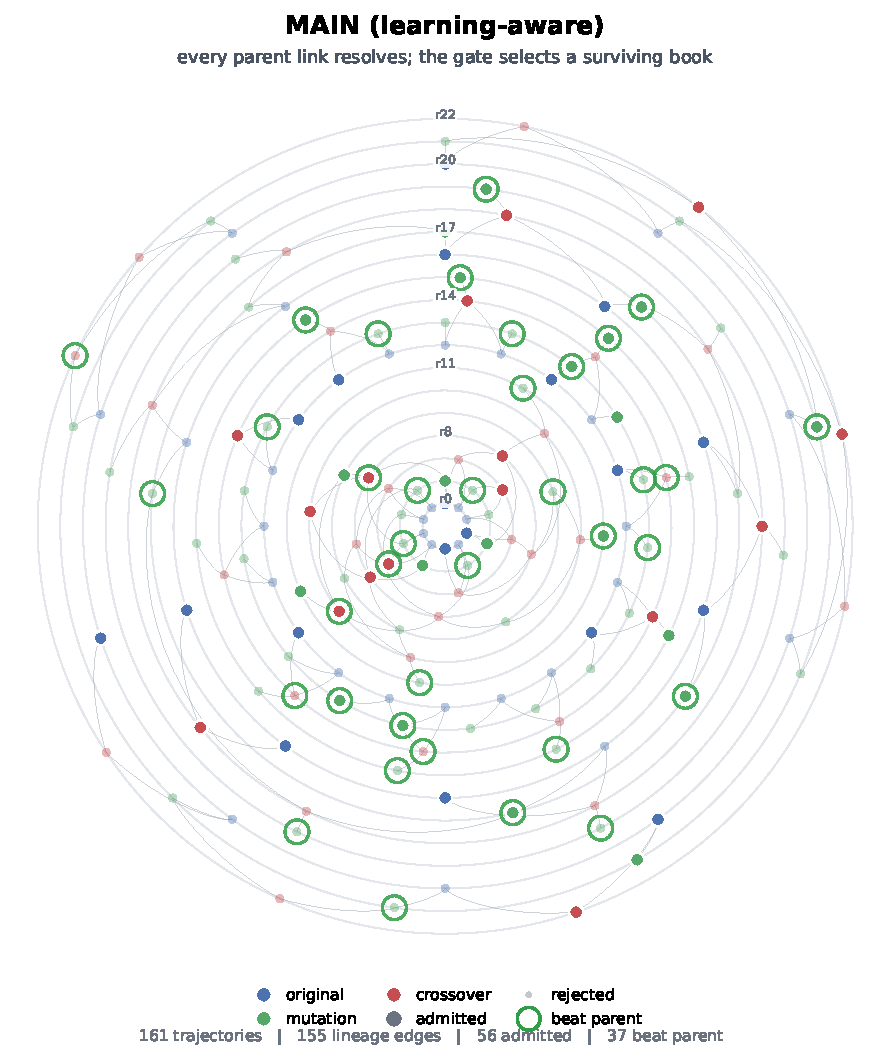
\includegraphics[width=\textwidth]{figures/fig_trajectory_main.pdf}
 \caption{\main{}: 161 trajectories over 18 rounds, 155 lineage links, 56 admitted,
 37 children beating their best parent.}
\end{subfigure}
\hfill
\begin{subfigure}[t]{0.49\textwidth}
 \centering
 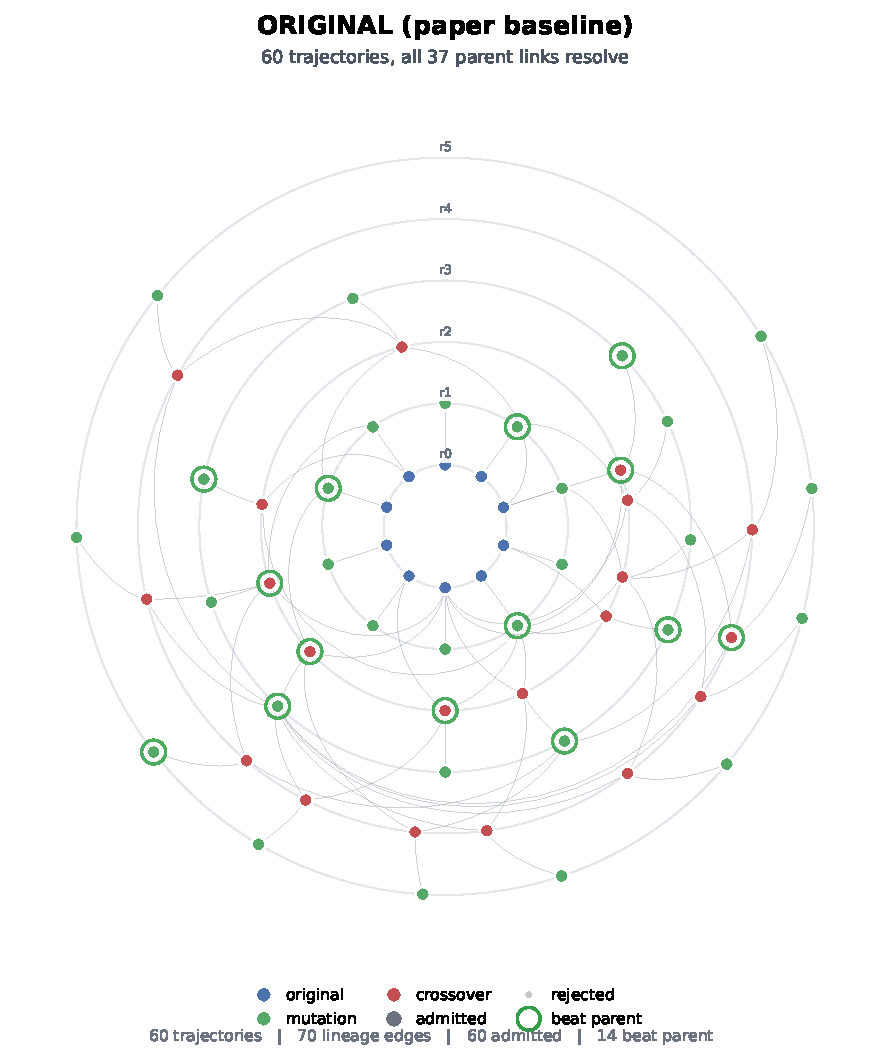
\includegraphics[width=\textwidth]{figures/fig_trajectory_original.pdf}
 \caption{\orig{}: 60 trajectories over 6 rounds, 70 lineage links, no admission
 step, 14 children beating their best parent.}
\end{subfigure}
\caption{Trajectory lineage: each ring is a round, each dot a formula, each curve a
parent-to-child link. \textbf{Conclusion: both searches are fully traceable, but only
\main{}'s is \emph{selective} --- its kept formulas (filled dots) keep appearing in the
outermost rings, so the search is still finding things worth keeping late in the run,
whereas \orig{} keeps everything and its tree simply widens.}}
\label{fig:traj}
\end{figure}

Three things are visible. \main{}'s admitted nodes are a minority scattered through
every ring rather than clustered early --- the gate keeps finding factors worth
keeping late in the run, which is what lets the accumulated book improve
(\S\ref{sec:learning}) while per-factor quality stays flat. \main{} runs eighteen
rounds to \orig{}'s six, but that follows from factor yield rather than search depth
(\S\ref{sub:budget}): both reach the same maximum breeding depth of five generations,
so \main{}'s extra rounds buy more distinct hypotheses (161 against 60), not a longer
chain of inheritance. And green halos --- children beating their best parent ---
appear throughout \main{}'s tree on both operators (37 of 111 bred children) but are
sparser in \orig{} (14 of 48), below what chance alone would give.

A ring does not mean the same thing in the two panels --- about ten factors in
\main{}, thirty in \orig{} --- so the panels compare on structure, not ring count.
\main{}'s rounds 3--7 are absent because the production run was resumed after a
mid-run model rollback; rings are indexed by ordinal position, so the gap leaves no
blank ring.

\section{Discussion}

\paragraph{What holds up.}
\main{} gets measurably better as it searches: the prediction quality of its formulas
rises six times faster than the baseline's (Table~\ref{tab:perfactor}), starting level
and finishing $53\%$ ahead. Compared at the same number of formulas, its generator
produces the better raw material. Over 2017--2025 it wins on both backtests ($+35.5\%$ against $+20.9\%$ a
year under simple costs, $+9.6\%$ against $+3.1\%$ under realistic ones), predicts
better in all nine years, loses less at its worst, and has by far the best trading
capacity --- beating \orig{} by $4$--$5$ percentage points a year at every fund size
once the fund is allowed to compound. It holds more genuinely different ideas and spreads them
across a wider range of building blocks. Its selection process demonstrably learns:
the portfolio it assembles improves steadily even as the statistical bar for admission
rises, every one of its 29 replacements beat the formula it displaced, and it never
kept a formula whose real behaviour contradicted the story it told. Its breeding beats
what it breeds from $53$--$61\%$ of the time, where the baseline's does so less often
than chance.

\paragraph{What does not.}
\main{}'s kept set predicts slightly worse than a random 56 drawn from its own library,
and its members are more similar to each other than in either full library --- the gate
buys portfolio contribution at some cost in raw prediction, and against its own library
that trade is currently about a wash. Reporting how formulas behave in crashes has not
yet produced a more crash-resistant library. And nothing is profitable on 2022--2025 at
any fund size. Note also that \main{}'s size-neutralised prediction score, which strips
out any edge coming from simply favouring small stocks, improves far less clearly than
its raw score.

\paragraph{Where the loss sits.}
The formulas predict well: every library scores positively every year across the whole
period, and under the simple merging model \main{}-full makes money in all nine. The
failure is downstream. The two backtests disagree not only on returns but on
\emph{prediction} --- $0.09$--$0.13$ against $0.03$--$0.06$ after 2020, on identical
formulas over identical days. No cost model can cause that, because prediction has no
costs in it. Both build the portfolio identically. The only remaining difference is
the model that merges many formulas into one score, and that is where the value is
being lost.

\paragraph{Three traps worth remembering.}
Each one, uncorrected, reverses a headline. The realistic setup measured the market
with an index that excludes dividends while the portfolio's returns include them,
crediting the strategy with the market's dividend yield as skill --- prediction scores
are immune, since they compare stocks within a day. The two systems' own stored numbers
were computed under different cost assumptions on different years and must never be
placed side by side. And the merging model improves simply from being given more
formulas, so any comparison that does not hold the count fixed penalises the more
selective system.

\section{Which System Is Better?}
\label{sec:verdict}

\textbf{\main{}, on the evidence collected here.} It is ahead on thirteen of the
fifteen measures in Table~\ref{tab:metrics}, and ahead on the ones that matter most:

\begin{itemize}[leftmargin=1.4em,itemsep=0.15em]
  \item \textbf{It learns, and the baseline barely does.} Formula quality improves six
        times faster ($+0.0236$ against $+0.0038$ Rank IC per hundred formulas). \main{}
        starts level and finishes $53\%$ ahead.
  \item \textbf{Its breeding works.} New formulas beat the ones they were bred from
        $53$--$61\%$ of the time; the baseline's do so \emph{less} often than chance
        ($21$--$28\%$), meaning its breeding usually destroys value.
  \item \textbf{Better portfolios, on both backtests, in every year.} $+35.5\%$ against
        $+20.9\%$ a year under simple costs and $+9.6\%$ against $+3.1\%$ under
        realistic ones over 2017--2025, with a higher prediction score in all nine years
        and a smaller worst-case loss ($-7.9\%$ against $-10.6\%$).
  \item \textbf{It scales better.} Run as a fund that starts at 100M and compounds, it
        beats the market by $7.84\%$ a year against the baseline's $2.40\%$, and holds
        that lead at every fund size.
  \item \textbf{It explored more.} The same 150 formulas cost \main{} 161 distinct ideas
        and \orig{} only 60, so \main{}'s result comes from genuinely wider search
        rather than variations on fewer thoughts.
\end{itemize}

\noindent \textbf{Where the baseline wins.} \orig{}'s formulas are marginally cheaper
to trade ($5.49$ against $5.81$ basis points) and hold their edge slightly better in
market crashes ($0.058$ against $0.054$). Judged one formula at a time on its own
recorded scores its formulas also look stronger --- but that is the flip side of a
selection rule that deliberately prefers formulas which add something new to the
portfolio over formulas that merely look good alone.

\noindent \textbf{The honest qualifications.} \main{}'s advantage is established on a
single run of each system, so some of the gap could be luck in what the language model
happened to propose; and neither system produces a strategy that is profitable under
realistic costs on the most recent four years. The first is addressed by the repeated
runs proposed below, the second by fixing the merging model.

\section{Next Steps}
\label{sec:next}

Ordered by effort, quickest first.

\begin{enumerate}[leftmargin=1.6em,itemsep=0.3em]
  \item \textbf{Re-run both systems on identical splits.} The seven-versus-one-year gap
        between tuning periods (\S\ref{sec:intro}) was an oversight and works against
        \main{}. Removing it makes every comparison in this report cleaner, and costs
        only the compute to re-mine.
  \item \textbf{Measure generation luck: three to five runs of each system.} Every
        result here rests on one run apiece. Repeating both and reporting the spread
        establishes whether \main{}'s margin exceeds run-to-run variation --- without
        which no single-run difference can be called real.
  \item \textbf{Test on the S\&P 500, two ways.} First, mine and test on US data, to see
        whether the advantage is a property of the method or of this market. Second,
        mine on CSI300 and test on the S\&P without re-mining --- a strict
        out-of-sample test of whether the formulas capture something general rather
        than something local.
  \item \textbf{Re-mine and re-test over a longer window, on both backtests.} This
        settles the open decay question: does \main{} still lead over a longer horizon,
        and does its edge resist decay better than the baseline's, under both simple
        and realistic costs?
  \item \textbf{Add continuous learning and a falsification critic.} The current system
        learns within a run; carrying that across runs is the natural extension. A
        critic that actively tries to \emph{disprove} each proposed formula would attack
        the weakness this report identifies --- the generator's raw output quality,
        the one thing that has not improved.
  \item \textbf{Fix the merging model and the portfolio constructor.} The largest and
        hardest item, and the one that binds everything else: prediction quality is
        good, yet the realistic path turns negative after 2020 and the two backtests
        disagree on prediction itself (\S\ref{sub:long}). Replacing the merging model
        with a properly specified one and the position builder with an industry-standard
        mean-variance construction is what stands between a demonstrated edge and a
        strategy worth running. Until it is done, no amount of generator improvement
        will show up in the returns.
\end{enumerate}

\end{document}
